% !TeX program = xelatex
% 16:9 aspect ratio 
\documentclass[aspectratio=169, 16pt]{beamer}
% remove the tool part that popups
\setbeamertemplate{navigation symbols}{}
\usepackage{physics}
\usepackage{etoolbox}
\usepackage{anyfontsize}
\usepackage{geometry}
\usepackage{fontspec}
\setmainfont{Arial}
\usepackage{xcolor}
\usepackage{pgfplots}
\usepgfplotslibrary{dateplot}
\pgfplotsset{compat=1.15}
\usepackage{hyperref}
\usepackage{xspace}
\usepackage[absolute,overlay]{textpos}
\usepackage{media9}
\usepackage{amsmath}
\usepackage{amssymb}
\usepackage{amsfonts}
\usepackage{tabu}
\tabulinesep = 1.5mm
% INL primary palette
\usepackage{subfiles} % Best loaded last in the preamble

% command for partial derivative
\newcommand{\pdiff}[2]{
    \frac{\partial #1}{\partial #2}
}
% command for a derivative
\newcommand{\diff}[2]{
    \frac{d #1}{d #2}
}
\newcommand{\unit}[1]{
    \: \left[ \text{#1} \right]
}
\newcommand{\fracunit}[2]{
    \: \left[
    \frac{\text{#1}}{\text{#2}}
    \right]
}

\setbeamertemplate{section title}{}

% Set the frame title backgrounds to be text black, background white
\setbeamercolor{palette primary}{fg=black, bg=white}

% Set the bar underneath the title blocks to a color
\setbeamercolor{progress bar}{fg=white,bg=white}

% Set text color
\setbeamercolor{normal text}{fg =black, bg=white}

% Set slide title color
\setbeamercolor{frametitle}{fg=black,bg=white}

% Global background set, to use the default frame background
\usebackgroundtemplate{
  \begin{picture}(0,0)
    \put(0,-\paperheight){
\includegraphics[width=\paperwidth,height=\paperheight]{figs/ncsu_slide_background.pdf}}
  \end{picture}
}

% removes the footnote line that is usually inserted
\renewcommand*\footnoterule{}
% removes auto formatted frame number so we can redefine them
\setbeamertemplate{frame numbering}[none]
% defines how the footnote on every slide is defined
\setbeamertemplate{footline}
{
  \leavevmode%
  \hbox{%
  % displayin the primary author and a short presentation name
  \begin{beamercolorbox}[wd=.9\paperwidth,ht=2.25ex,dp=1ex,left]{author in head/foot}%
    \hspace*{2ex} 
    \usebeamerfont{author in head/foot}\insertshortauthor - \insertshorttitle 
  \end{beamercolorbox}%
  % adding the page numbers
  \begin{beamercolorbox}[wd=.1\paperwidth,ht=2.25ex,dp=1ex,right]{author in head/foot}%
    \insertframenumber{} \hspace*{2ex} 
  \end{beamercolorbox}}%
  \vspace{0.5em}
}

\usepackage[
  backend=biber,
  style=verbose-note,
  autocite=footnote,
  citetracker=true, 
  giveninits=true, 
  uniquename=init
]{biblatex}
\setbeamertemplate{bibliography item}{}

\newtoggle{citeseen}

\newbibmacro{cite:extrainfo:article}{%
  \printnames[family-given][1-1]{labelname}
  \newunit
  \usebibmacro{journal}
  \newunit 
  \printfield{year}
}

\newbibmacro{cite:extrainfo:book}{%
  \printnames[family-given][1-1]{labelname}%
  \newunit
  \printfield{title}%
}

\newbibmacro{cite:extrainfo:techreport}{%
  \printnames[family-given][1-1]{labelname}%
  \newunit
  \printfield{title}%
}

% TODO: fix the techreport citation 
\renewbibmacro*{cite}{%
  \ifboolexpr{
    test {\ifentrytype{article}}
    or
    test {\ifentrytype{book}}
    or
    test {\ifentrytype{techreport}}
  }{%
    \ifciteseen{%
      \iftoggle{citeseen}{%
        \textsuperscript{\thefootnote}%
      }{%
        \mkbibfootnote{%
          \ifentrytype{article}
            {\usebibmacro{cite:extrainfo:article}}{}
          \ifentrytype{book}
            {\usebibmacro{cite:extrainfo:book}}{}
          \ifentrytype{techreport}
            {\usebibmacro{cite:extrainfo:techreport}}{}
        }%
        \global\toggletrue{citeseen}%
      }%
    }{%
      \mkbibfootnote{%
          \ifentrytype{article}
            {\usebibmacro{cite:extrainfo:article}}{}
          \ifentrytype{book}
            {\usebibmacro{cite:extrainfo:book}}{}
          \ifentrytype{techreport}
            {\usebibmacro{cite:extrainfo:techreport}}{}
      }%
      \global\toggletrue{citeseen}%
    }%
  }{}%
}


    
% Remove the page icon and number from the bibliography
\DeclareFieldFormat{pages}{}
\DeclareFieldFormat{postnote}{}
\renewbibmacro*{pageref}{}
% Load the bibliography file
\addbibresource{works.bib}

% Customize the frametitle template to remove the progress bar
\setbeamertemplate{frametitle}{%
  \nointerlineskip%
  \usebeamerfont{frametitle}%
  \begin{minipage}[b][2.5ex][c]{\textwidth}
    \vspace*{2.5cm}
    \centering
    \textbf{\insertframetitle}%
  \end{minipage}%
}

% setting fontsizes typically 1/2 of pptx size is the same

\renewcommand{\small}{\fontsize{10}{12}\selectfont}
\renewcommand{\normalsize}{\fontsize{10}{12}\selectfont}
\renewcommand{\large}{\fontsize{11}{13.2}\selectfont}
\renewcommand{\huge}{\fontsize{20}{24}\selectfont}


\makeatletter
% Command to set the first author
\newcommand{\firstauthor}[1]{%
  \gdef\@firstauthor{#1}%
}

% Command to insert the first author
\newcommand{\insertfirstauthor}{%
  \@ifundefined{@firstauthor}
    {\@latex@warning@no@line{First author not set}}
    {\textbf{\underline{\smash{\@firstauthor}}}}%
}

\newcommand{\insertplainfirstauthor}{%
  \@ifundefined{@firstauthor}
    {\@latex@warning@no@line{First author not set}}
    {\@firstauthor}
}
% Initialize first author to empty
\gdef\@firstauthor{}

\newcommand{\advisor}[1]{%
  \gdef\@advisor{#1}%
}

\newcommand{\insertadvisor}{%
  \@ifundefined{@advisor}
    {\@latex@warning@no@line{First author not set}}
    {\textbf{\underline{\smash{\@advisor}}}}%
}

\gdef\@advisor{}
\makeatother
% Short title, which will be displaed on every slide
\title[MOOSE Based Kinetic Plasma Simulation Verification]
{
}

\firstauthor{Grayson Gall}
\advisor{Amanda Lietz}
% short author, this is what will be displayed on every slide
\author[\insertplainfirstauthor]{}
\setbeamertemplate{background canvas}{%
    
\includegraphics[width=\paperwidth,height=\paperheight]{figs/ncsu_slide_background.pdf}%
}
% setting the markers in the itemize environment to be bullets
\setbeamertemplate{itemize item}{\centering\textcolor{black}{$\bullet$}}
\setbeamertemplate{itemize subitem}{\centering\textcolor{black}{$\bullet$}}
\setbeamertemplate{itemize subsubitem}{\centering\textcolor{black}{$\bullet$}}

\setbeamerfont{itemize item}{family=\centering}
\setbeamerfont{itemize subitem}{family=\centering}
\setbeamerfont{itemize subsubitem}{family=\centering}

\AtBeginSection[]{
  \begingroup
  \setbeamercolor{section in toc}{fg=black}
  \begin{frame}
    \tableofcontents[currentsection]
  \end{frame}
  \endgroup
}

\begin{document}
%
% Title slide
%
% set the background for the title slide to be different if needed 
\begin{frame}[plain]
   \hspace*{-0.25in}
   \vspace{-1.5cm}
    \begin{minipage}{\dimexpr\textwidth+0.5in\relax} % Adjust 2cm as needed
      \centering
      {\huge\textbf{
% Full title for the talk 
      Kinetic Plasma Simulation in the MOOSE\\
      Framework: Verification of Electrostatic\\
      Particle In Cell Capabilities\\
      }\vspace{\baselineskip}}
      \insertfirstauthor$^\mathbf{1}${\large \textbf{,}}
      {\large \textbf{Logan H. Harbour$^{\mathbf{2}}$,
      Casey T. Icenhour$^{\mathbf{2}}$, 
      Pierre-Clément A. Simon$^{\mathbf{2}}$,\\
      Derek Gaston$^{\mathbf{2}}$,}}
      \insertadvisor$^{\mathbf{1}}$\\
      {\large \vspace{\baselineskip}}
      {\normalsize \textbf{$^\mathbf{1}$North Carolina State University, Raleigh, North Carolina\\ ${^\mathbf{2}}$Idaho National Laboratory, Idaho Falls, Idaho}\\ \vspace{\baselineskip}}
      {\large \textbf{Pacific Basin Nuclear Conference 2024}\\ \vspace{\baselineskip}}
      {\normalsize \textbf{Supported by the Idaho National Laboratory, Laboratory Directed Research \& Development (LDRD) Program}}
    \end{minipage}
\end{frame}

\addtocounter{framenumber}{-1}
\section{Motivation and Background}
\begin{frame}{Motivation}
  \vfill{}
  \begin{itemize}
    \item In recent years, Fusion energy has gained significant interest and funding.
    \begin{itemize}
      \item Several fusion energy companies are targeting 2030 as the goal for energy generation.
    \end{itemize}
    \item However, the design plasma facing components (PFCs) is particularly challenging.
    \begin{itemize}
      \item PFCs exist in a highly coupled multiphysics environment.
      \item Experimental data is rare and expensive.
    \end{itemize}
    \item In order to meet this challenge scalable multiphysics frameworks are required\cite{carter2020powering}.
    \begin{itemize}
      \item To address this need kinetic plasma modeling capabilities are being developed as a part of the Fusion ENergy Integrated multiphys-X (FENIX) framework.
      \item FENIX benefits from all of the flexiblity and scalability of the MOOSE framework.
    \end{itemize}
  \end{itemize}
\end{frame}

\begin{frame}{Particle-In-Cell}
  \vfill{}
  \begin{itemize}
    \item Individual computational particles that represent multiple physical particles are tracked.
    \begin{itemize}
      \item In FENIX this is build on MOOSE's Ray Tracing module.
    \end{itemize}
    \item Maxwell's equations are solved based on computational particle positions and path. 
    \begin{itemize}
      \item Typically, finite difference solvers with uniform grids are used.
    \end{itemize}
    \item FENIX is built on top of the MOOSE framework, this enables
    \begin{itemize}
      \item Finite element based simulations.
      \item 1D,2D, or 3D simulations.
      \item Non-uniform domain discritizations.
      \item Massive parallelization.
      \item Rhobust software quality assurance and testing.
      \item Coupling with other physics modules.
    \end{itemize}
  \end{itemize}
\end{frame}

\begin{frame}
  \vspace{0.5cm}
  \begin{figure}[H]
    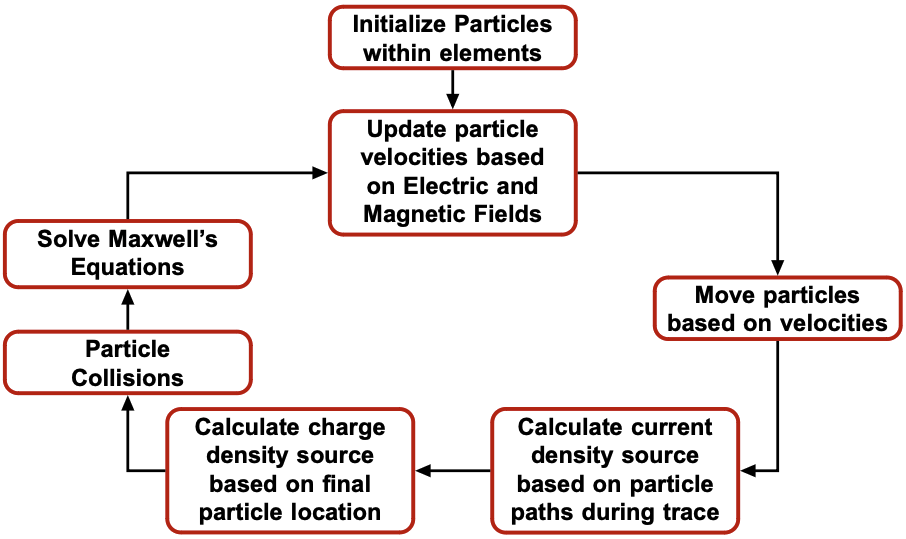
\includegraphics[height=0.8\textheight]{figs/flowchart.png}
  \end{figure}
\end{frame}

\section{Mathematics and Verification}

\begin{frame}{Verification Motivation}
  \vfill{}
  \begin{itemize}
    \item Rigorous verification denomstrates the proper implemenation of FENIX's PIC capabilities.
    \begin{itemize}
      \item Gives researchers a higher degree of confidence when exploring new devices/regimes.
      \item Enables an easier road for licensing of designs based on FENIX calculations.
    \end{itemize}
    \item PIC is heavily utilized by the Low Temperature Plasma (LTP) community.
    \begin{itemize}
      \item Verification studies are not prioritized and are rarely published in the LTP community\cite{alves2023foundations}.
    \end{itemize}
  \end{itemize}
\end{frame}

\begin{frame}{Particle Description}
    \vfill{}
    \begin{itemize}
      \item FENIX treats computational particles as point particles.
    \end{itemize}
    \begin{align}
      f \left( \vec{r}, \vec{v}, t \right) 
      =
      \sum_{i=1}^N 
      \omega_i q_i 
      \delta \left( \vec{r} - \vec{r}_i(t) \right)
      \delta \left( \vec{v} - \vec{v}_i(t) \right)
    \end{align}
    \begin{columns}
      \column{0.5\textwidth}
      \begin{itemize}
        \item $f\;$: Particle distribution function.
        \item $N\;$: Computational particle count. 
        \item $\omega_i\;$: Computational particle weight.
        \item $q_i\;$: Computational particle charge.
      \end{itemize} 
      \column{0.5\textwidth}
      \begin{itemize}
        \item $\delta\;$: Dirac Delta Function.
        \item $\vec{r}\;$: Particle position.
        \item $\vec{v}\;$: Particle velocity
        \item $t\;$: Simulation time
      \end{itemize}
    \end{columns}
\end{frame}

\begin{frame}{Single Particle Motion}
  \vfill{}
  \centering
  The equations of motion are solved for each computational particle, individually.
    \centering
      \begin{equation}
        \diff{\,\vec{r}}{t}
        =
        \vec{v}
      \end{equation}
      \begin{equation}
          \diff{\,\vec{v}}{t}
          =
          \frac{q}{m}
          \left(
            \vec{E} +
            \vec{v} \times
            \vec{B}
          \right)
      \end{equation}
    $\vec{E}$ and $\vec{B}$ represent the electric and magnetic fields repsectively.
\end{frame}

\begin{frame}{Leapfrog Particle Stepping}
  \begin{figure}[H]
    \centering
    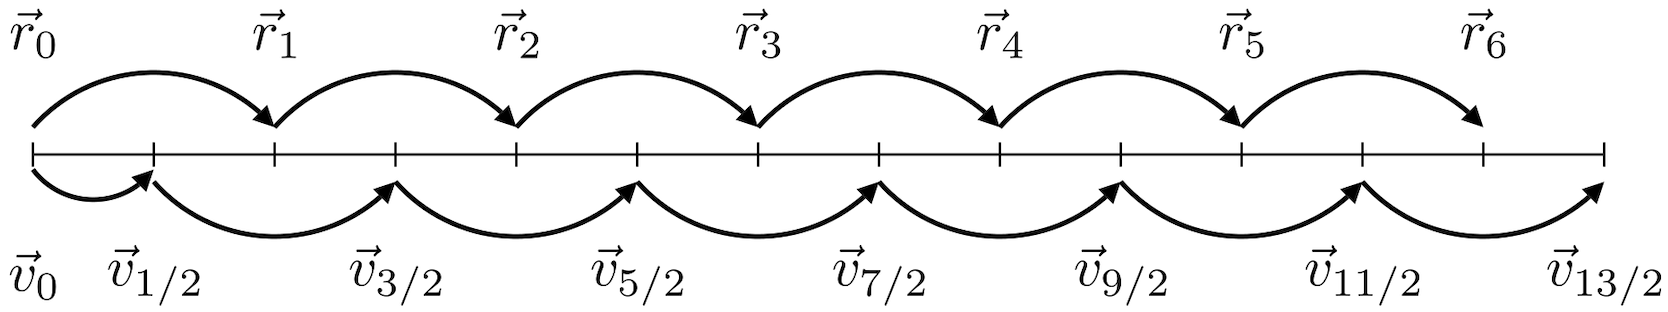
\includegraphics[width=\textwidth]{figs/BorisVisualization.png}
  \end{figure}
\end{frame}


\begin{frame}{Boris Stepping}
  \vfill{}
  \centering
  Particles are stepped through electromagnetic fields using the boris algorithm\cite{boris1970relativistic}.
  \vspace{0.25cm}
  \begin{columns}
    \column{0.5\textwidth}
      \begin{equation} \label{eq:e_half1} \vec{v}^{\,-}
        =
        \vec{v}_{n}
        +
        \frac{q}{m}
        \vec{E}_n
        \frac{\Delta t}{2}
      \end{equation}
      \begin{equation} \label{eq:boris_v_plus}
        \vec{v}^{\,+}
        =
        \vec{v}^{\,-}
        +
        \vec{v}^{\,'}
        \times
        \vec{s}
      \end{equation}
      \begin{equation} \label{eq:boris_v_prime}
        \vec{v}^{\,'}
        =
        \vec{v}^{\,-}
        +
        \vec{v}^{\,-}
        \times
        \vec{l}
      \end{equation}
      \begin{equation} \label{eq:boris_t}
        \vec{l} =
        \frac{q}{m}
        \vec{B}_n
        \Delta t
      \end{equation}
      \column{0.5\textwidth}
      \begin{equation} \label{eq:boris_s}
        \vec{s} =
        \frac{2 \vec{l}}{
          1 + \vec{l} \cdot \vec{l}
        }
      \end{equation}
      \begin{equation} \label{eq:mag_step}
        \frac{
          \vec{v}^{\,+}
          -
          \vec{v}^{\,-}
        }{ \Delta t}
        =
        \frac{q}{m}
        \left(
          \vec{v}^{\,+}
          +
          \vec{v}^{\,-}
        \right)
        \times
        \vec{B}_n
      \end{equation}
      \begin{equation} \label{eq:e_half2}
        \vec{v}_{n+1}
        =
        \vec{v}^{\,+}
        +
        \frac{q}{m}
        \vec{E}_n
        \frac{\Delta t}{2}
      \end{equation}
  \end{columns}
  \vspace{0.25cm}
  $\vec{E}$ and $\vec{B}$ represent the electric and magnetic fields respecitvely, and $n$ is denotes the number of the current timestep.
\end{frame}

\begin{frame}{Cyclotron Motion}
  \vfill{}
  \begin{columns}
    \centering
    \column{0.5\textwidth}
    \begin{itemize}
      \item A single particle in the magnetic field given by $\vec{B} = 1 \hat{z}$
      \item Particle Properties:
      \begin{itemize}
        \item $q = 1 \unit{C}$
        \item $m  = 1 \unit{kg}$ 
        \item $\omega = 1 \fracunit{1}{m}$
        \item $v_\perp = 1 \fracunit{m}{s}$
      \end{itemize}
    \end{itemize}
    $v_\perp$ is the magnitude of the velocity perpendicular to the magnetic field.
    \column{0.5\textwidth}
      \begin{figure}[H]
        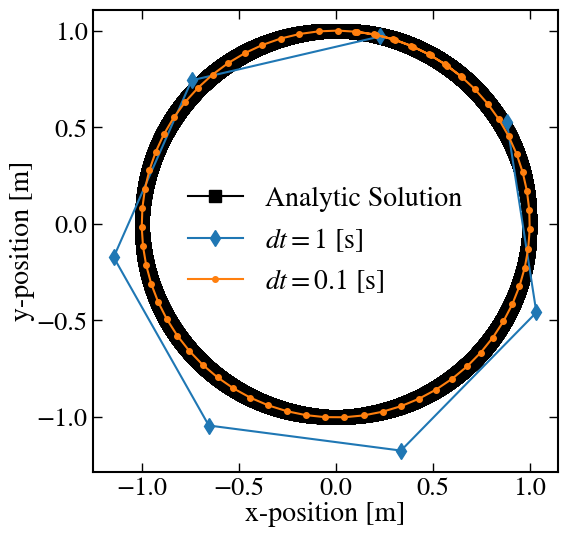
\includegraphics[width=0.9\textwidth]{figs/cyclotron.png}
      \end{figure}
  \end{columns}
\end{frame}

\begin{frame}{Cyclotron Motion Errors}
  \vfill{}
  \begin{columns}
    \centering
    \column{0.5\textwidth}
      \begin{figure}[H]
        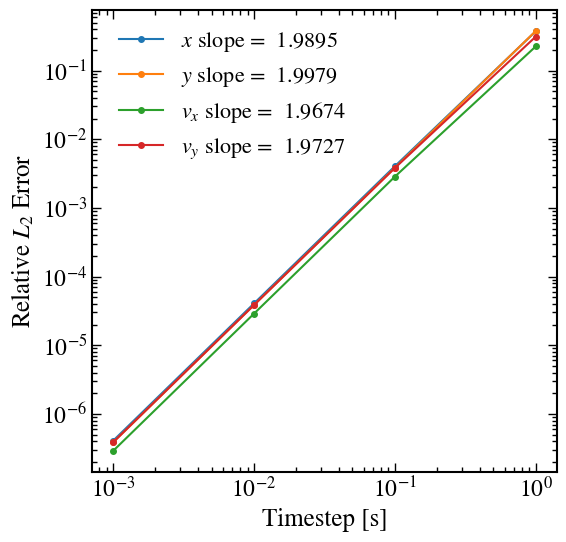
\includegraphics[width=0.9\textwidth]{figs/cyclotron_l2_error.png}
      \end{figure}
    \column{0.5\textwidth}
      \begin{figure}[H]
        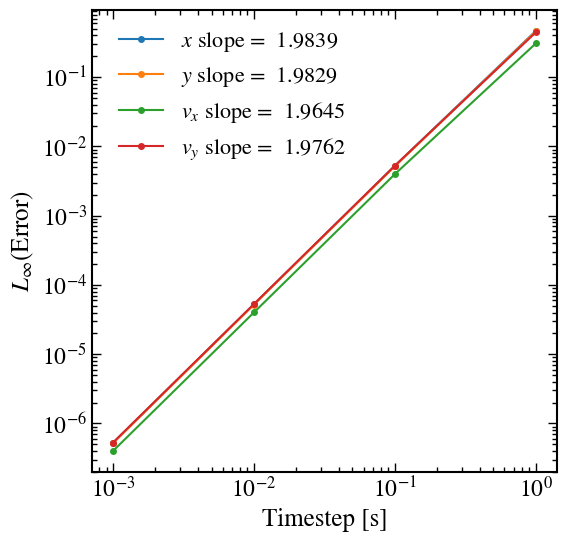
\includegraphics[width=0.9\textwidth]{figs/cyclotron_error.png}
      \end{figure}
  \end{columns}
\end{frame}

\begin{frame}{Charge Density Calculation}
    \vspace{0.75cm}
    \begin{equation}
      \left< \, 
      \rho(\vec{r}\,), 
      \phi_i(\vec{r}\,)
      \right> 
      = 
      \sum_{j=1}^{N_i} 
      q_j\,
      \omega_j\,
      \psi
      \left( \vec{r} - \vec{r}_j
      \right) 
    \end{equation}
    \vspace{-0.75cm}
  \begin{columns}
    \column{0.5\textwidth}
    \begin{itemize}
      \item Solving for the electric field requires solving Poisson's equation.
    \end{itemize}
    \begin{align}
      \laplacian \phi = \frac{ \rho }{ \varepsilon_0 }
    \end{align}
    \begin{itemize}
      \item This requies evaluating the inner product of the computational charge distribution and the basis functions, $\psi$
    \end{itemize}
    \column{0.5\textwidth}
    \begin{figure}[H]
      \centering 
      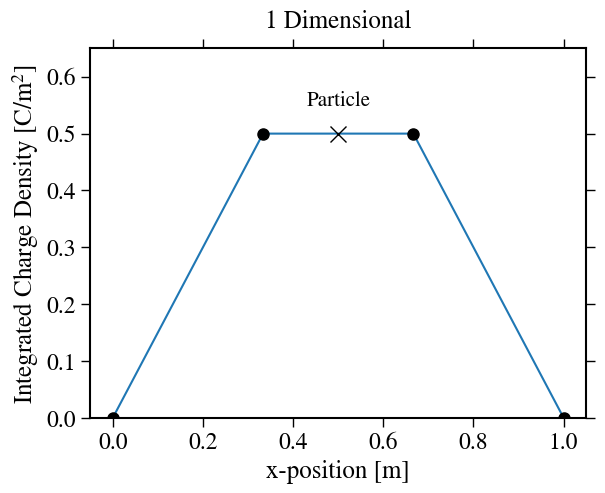
\includegraphics[width=0.8\textwidth]{figs/charge_1D.png}
    \end{figure}
  \end{columns}
\end{frame}

\begin{frame}{Particle Initialization}
  \vspace{1cm}
  \begin{columns}
    \column{0.5\textwidth}
      \begin{itemize}
        \item A widely used initial condition for particles is a uniform distribution throughout the domain.
        \begin{itemize}
          \item In FENIX each elements volume is uniformly sampled.
        \end{itemize}
      \item Initial particle position is a randomly sample quantity so the error in the projection of the particle density onto the mesh follows a standard sample variance.
      \end{itemize}
      \begin{align}
        S^2 = 
        \frac{ 1 }{ N - 1 }
        \sum_{i=1}^N 
        \left( x_i - \overline{x} \right)^2
      \end{align}
    \column{0.5\textwidth}
      \centering 
      \begin{figure}
        \centering 
        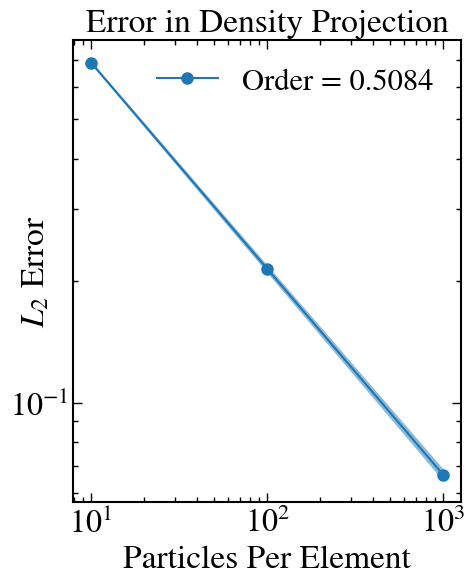
\includegraphics[height=0.7\textheight]{figs/density_error.png}
      \end{figure}
  \end{columns}
  
\end{frame}

\begin{frame}{Electrostatic Potential}
  \vfill{}
  \begin{columns}
    \column{0.5\textwidth}
    \begin{figure}[H]
      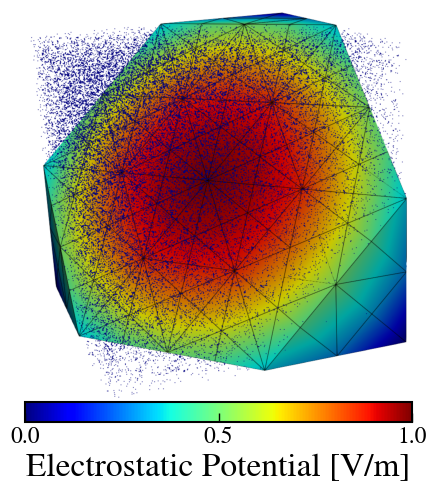
\includegraphics[width=0.7\textwidth]{figs/potential_visualiation.png}
     \end{figure}
    \column{0.5\textwidth}
    \begin{figure}[H]
      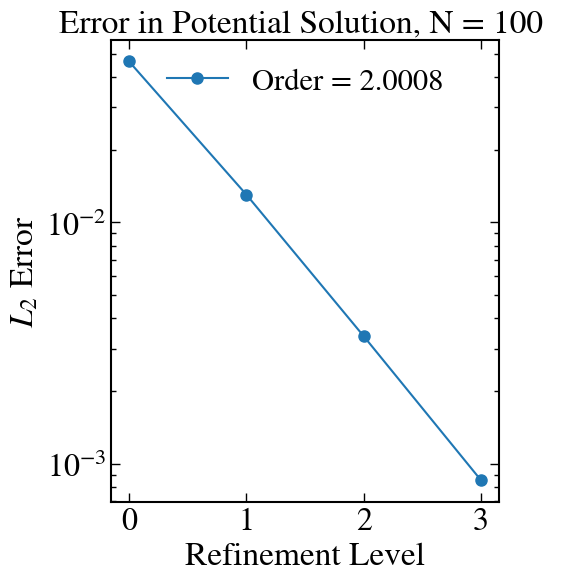
\includegraphics[width=0.8\textwidth]{figs/potential_error.png}
     \end{figure}
  \end{columns}
\end{frame}

\begin{frame}{Current Density}
      \begin{align}
        \left<
          \vec{J}_{n + 1/2}
          \left(\vec{r}, t\right),
          \vec{\psi}(\vec{r}\,)
          \right> =
        \frac{1}{\Delta t}
        \int_{t_n}^{t_{n+1}}
        \sum_{i=1}^N
        q_i \,\omega_i
        \vec{v}_i(t)
        \cdot
        \vec{\psi}(\vec{r}_i(t))
        dt
      \end{align}
  \begin{columns}
    \column{0.5\textwidth}
      \begin{itemize}
        \item Current density is often a parameter of interest and is required to solve the full set of Maxwell's equations
      \end{itemize}
      \begin{align}
        \pdiff{\rho}{t} &= - \div \vec{J}\\
        \left< \rho_1 - \rho_0, \psi \right> &= \Delta t \left< \vec{J}_{n + 1/2}, \grad \psi \right>
      \end{align}
    \column{0.5\textwidth}
    \begin{figure}
      \centering 
      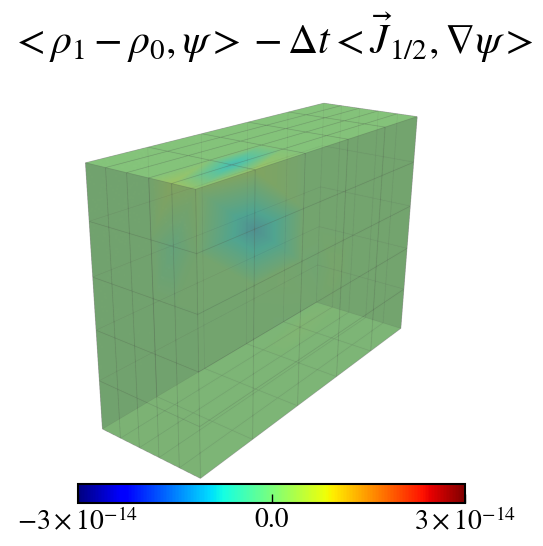
\includegraphics[height=0.5\textheight]{figs/conservation.png}
      \setlength{\unitlength}{1cm}
      \begin{picture}(0,0)
        \put(-2.65, 0){\makebox(0,0)[lt]{{\tiny[$C$\textbf{/}m$^2$]}}} % Add a textbox at coordinates (2,2)
      \end{picture}
    \end{figure}
  \end{columns}
\end{frame}

\begin{frame}{Lieberman Benchmark}
  \vfill{}
  \begin{columns}
    \column{0.33\textwidth}
    \begin{figure}[H]
      \centering
      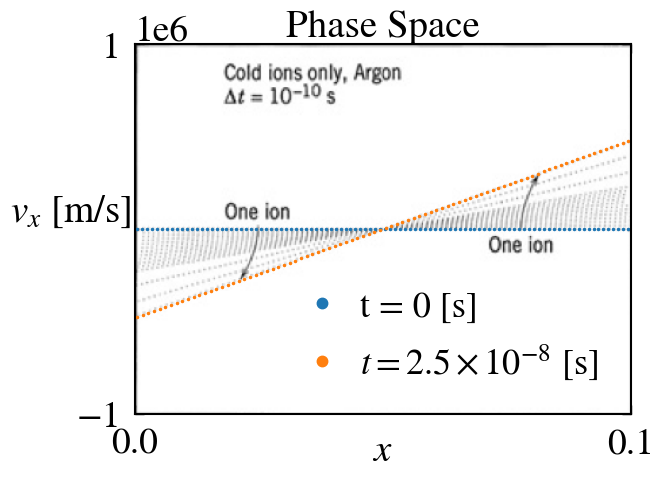
\includegraphics[width=\textwidth]{figs/lieberman_vdf_comparison.png}
    \end{figure}
    \column{0.33\textwidth}
    \begin{figure}[H]
      \centering
      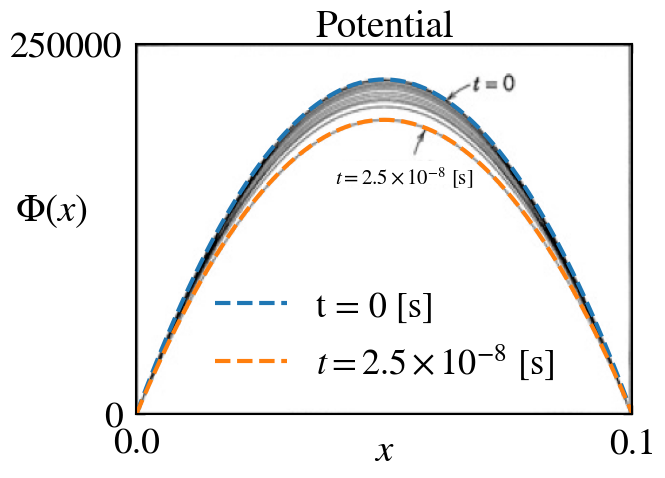
\includegraphics[width=\textwidth]{figs/lieberman_potential_comparison.png}
    \end{figure}
    \column{0.33\textwidth}
    \begin{figure}[H]
      \centering
      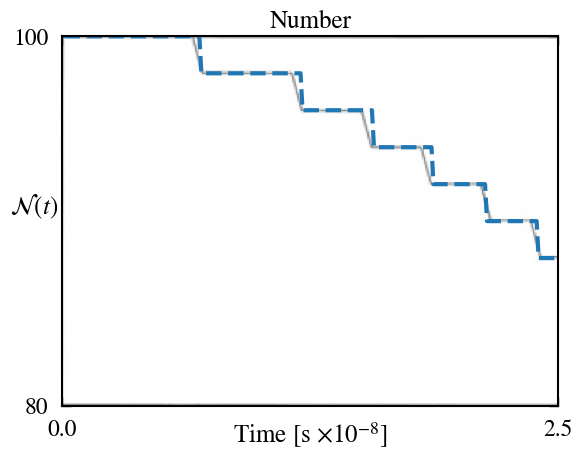
\includegraphics[width=\textwidth]{figs/lieberman_population_comparison.png}
    \end{figure}
  \end{columns}
    A simple collisionless single particle simulation demonstration from Lieberman\cite{lieberman2005} was replicated and documented as a training example.
\end{frame}

\section{Future Work}
\begin{frame}{Future Work} 
  \vfill{}
  \begin{itemize}
    \item Currently work is underway to demonstrate some canonical kinetic plasma instabilities:
    \begin{itemize}
      \item Landau Damping
      \item Two-stream instability
      \item Dory–Guest–Harris
    \end{itemize}
    \item Replication of an analytic solution applicable to both fluid and kinetic simulations\cite{lafleur2022space}.
    \item Particle-Particle collisions will be implemented.
    \item Computing heatfluxes from particle fluxes.
    \item Coupling with other MOOSE applications.
  \end{itemize}
\end{frame}

\section{Summary}
\begin{frame}{Summary}
  \vfill{}
  \begin{columns}
    \column{0.5\textwidth}
    \begin{itemize}
      \item The fundamental capabilities for PIC have been verified.
      \item FENIX will enable FEM PIC simulations within the MOOSE frameowork.
      \item FENIX can perform simulations in 1D, 2D, and 3D.
      \item FENIX will be one of the only openly available massively parallel kinetic plasma simulation tools.
      \item Rhobust verification enables FENIX to be able to utilized as an engineering tool.
    \end{itemize}
    \column{0.5\textwidth}
    \begin{figure}[H]
      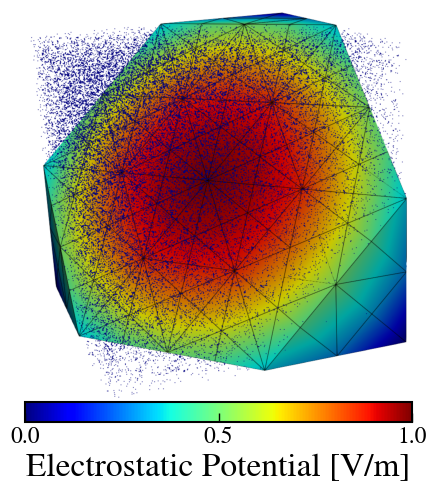
\includegraphics[width=0.7\textwidth]{figs/potential_visualiation.png}
     \end{figure}
  \end{columns}
\end{frame}
\begin{frame}
\end{frame}

\end{document}
